\documentclass[a4paper,12pt]{article}
\usepackage{tabularx}
\usepackage{amsmath}
\usepackage[utf8]{inputenc}
\usepackage{multicol}
\usepackage{cancel}
\usepackage{amsmath, amssymb, amsthm}
\usepackage{graphicx}
\usepackage{enumitem}
\usepackage{array}
\usepackage[left=2cm, right=2cm, top=2cm, bottom=2cm]{geometry}
\usepackage{fancyhdr}
\usepackage{xfp}
\usepackage{pgf}
\usepackage{tikz}

\usepackage{graphicx}
\usepackage{fancyhdr}

\setlength{\headheight}{28pt} % genug Platz für das Logo
\pagestyle{fancy}
\fancyhf{} % alles leeren
\fancyhead[L]{\includegraphics[height=1.2cm]{logo.png}}
\fancyhead[C]{\small Quadratische Funktionen \ (Kl. G9A)}
\fancyhead[R]{\small Name:\ \rule{2.8cm}{0.4pt}}
\fancyfoot[C]{\thepage}

\fancyfoot[C]{Seite \thepage \enspace\textbullet\enspace J.\,Mycan \textcopyright~17.Dez.2025 *Klassenarbeit 45 min.*}

\renewcommand{\footrulewidth}{0.4pt}

%\pagestyle{fancy}
%\lhead{Klassenarbeit 45min.}
%\chead{Heinrich-von-Kleist-Schule}
%\rhead{Mathematik - G8A}
%\lfoot{}
%\cfoot{Seite \thepage}
%\rfoot{}

\newcommand{\punkteA}{8}
\newcommand{\punkteB}{12}
\newcommand{\punkteC}{9}
\newcommand{\punkteD}{15}
\newcommand{\punkteE}{8}
%\newcommand{\punkteF}{22}

\newcommand{\maxSumme}{52}
\newcommand{\noteEinsMin}{\fpeval{round(\maxSumme * 0.95,0)}}
\newcommand{\noteZweiMin}{\fpeval{round(\maxSumme * 0.80,0)}}
\newcommand{\noteDreiMin}{\fpeval{round(\maxSumme * 0.60,0)}}
\newcommand{\noteVierMin}{\fpeval{round(\maxSumme * 0.45,0)}}
\newcommand{\noteFunfMin}{\fpeval{round(\maxSumme * 0.20,0)}}
\newcommand{\noteSechsMin}{0}

\newcommand{\summe}{%
	\pgfmathparse{\punkteA + \punkteB + \punkteC + \punkteD + \punkteE}%
	\pgfmathprintnumber{\pgfmathresult}}

\begin{document}
	
%	\begin{center}
%		\textbf{Klassenarbeit - Lineare Funktionen und LGS}
%	\end{center}
	
%	\textbf{Vor- und Nachname:} \underline{\hspace{10cm}}\\[0.1cm]
%\vspace{2cm}
	
%	\textbf{Vor- und Nachname:} \underline{\hspace{10cm}}\\[0.1cm]
%Die Lösungen sowie Lösungswege sollten klar strukturiert und gut nachvollziehbar sein. \\[0.1cm]
		% -------------------------------------------------
	% Aufgabe 1
	% -------------------------------------------------
	\textbf{Aufgabe 1 (8 Punkte)}\\
	Im folgenden Koordinatensystem sind vier verschiedene Parabeln eingezeichnet:
	\begin{center}
		\begin{minipage}{0.55\textwidth}
			\centering
			\begin{tikzpicture}[scale=0.9]
				% Koordinatensystem [-4,4] x [-4,4] mit Gitter
				\draw[step=1,very thin,gray!40] (-4,-4) grid (4,4);
				\draw[->] (-4,0) -- (4.3,0) node[right] {$x$};
				\draw[->] (0,-4) -- (0,4.3) node[above] {$y$};
				
				% Achsenbeschriftung
				\foreach \x in {-3,-2,-1,1,2,3}
				\draw (\x,0.1) -- (\x,-0.1) node[below=2pt] {\scriptsize \x};
				\foreach \y in {-3,-2,-1,1,2,3}
				\draw (0.1,\y) -- (-0.1,\y) node[left=2pt] {\scriptsize \y};
				
				% Graph I: f(x) = 1/4 x^2 - 2 (nach oben geöffnet, leicht nach unten verschoben)
				\draw[thick,domain=-4:4,smooth,variable=\x]
				plot ({\x},{0.25*\x*\x - 2});
				\node[font=\small] at (0,-2.4) {\textbf{I}};
				
				% Graph II: f(x) = 3/4 (x-1)^2 - 3 (nach oben, nach rechts/unten verschoben)
				\draw[thick,dashed,domain=-2:4,smooth,variable=\x]
				plot ({\x},{0.75*(\x-1)*(\x-1) - 3});
				\node[font=\small] at (1,-3.4) {\textbf{II}};
				
				% Graph III: f(x) = -1/4 x^2 + 3 (nach unten, nach oben verschoben)
				\draw[thick,dotted,domain=-4:4,smooth,variable=\x]
				plot ({\x},{-0.25*\x*\x + 3});
				\node[font=\small] at (0,3.4) {\textbf{III}};
				
				% Graph IV: f(x) = -3/4 (x+1)^2 + 3 (nach unten, nach links/oben verschoben)
				\draw[thick,densely dashed,domain=-4:2,smooth,variable=\x]
				plot ({\x},{-0.75*(\x+1)*(\x+1) + 3});
				\node[font=\small] at (-1,3.4) {\textbf{IV}};
				
			\end{tikzpicture}
		\end{minipage}%
		\hfill
		\begin{minipage}{0.4\textwidth}
			\small
			\textbf{Zuordnung:}\\[0.5em]
			Ordne jedem Graphen \textbf{I–IV} genau eine der folgenden
			Funktionsgleichungen zu.
			
			\begin{align*}
				\text{A)}\quad & f(x) = \tfrac{1}{4}x^{2} - 2 \\
				\text{B)}\quad & f(x) = \tfrac{3}{4}(x-1)^{2} - 3 \\
				\text{C)}\quad & f(x) = -\tfrac{1}{4}x^{2} + 3 \\
				\text{D)}\quad & f(x) = -\tfrac{3}{4}(x+1)^{2} + 3 \\
				\text{E)}\quad & f(x) = \tfrac{1}{2}x^{2} + 1
			\end{align*}
		\end{minipage}
	\end{center}
	
	% -------------------------------------------------
	% Aufgabe 2
	% -------------------------------------------------
\textbf{Aufgabe 2 (12 Punkte)}\\
Bestimme zu den folgenden Angaben jeweils die Funktionsgleichung einer
quadratischen Funktion in \emph{Scheitelpunktform}.

\begin{enumerate}
	\item[a)] Gegeben ist der Scheitelpunkt der Normalparabel \(S(-2\mid 3)\). 
	Stelle die Funktionsgleichung dieser Parabel in Scheitelpunktform auf.
	
	\item[b)] Gegeben ist die quadratische Funktion 
	\[
	f(x) = -1{,}5x^{2} - 12x + 18.
	\]
	Bringe \(f(x)\) in die Scheitelpunktform.
	
	\item[c)] Eine quadratische Funktion \(g\) besitzt die Nullstellen 
	\(x_1 = -1\) und \(x_2 = 5\) und hat den Streckfaktor \(a = 2\).\\
	Bestimme eine Funktionsgleichung von \(g\) in Scheitelpunktform.
\end{enumerate}

	
	% -------------------------------------------------
	% Aufgabe 3
	% -------------------------------------------------
\textbf{Aufgabe 3 (9 Punkte)}\\[0.3em]
Die Skizze rechts zeigt den Korbwurf eines Basketballspielers.\\
a) Welche der folgenden Funktionen gibt die dargestellte Flugbahn wieder?
Begründe \underline{\textbf{kurz}} deine Antwort.\\

\noindent
\begin{minipage}[t]{0.45\textwidth}
	\vspace{0pt}

\[
\begin{aligned}
	f(x) &= -2x^{2} + 12x - 14\\[2pt]
	g(x) &= 2x^{2} + 12x - 13\\[2pt]
	h(x) &= -2(x-4)^2 -1
\end{aligned}
\]


	\medskip
	b) Der Ball verließ die Hand des Spielers beim \(x\)-Wert \(2\). Wie hoch war die Hand beim Abwurf?\\[0.6em]
	c) Berechne den höchsten Punkt der Flugbahn des Balles.
\end{minipage}%
\hfill
\begin{minipage}[t]{0.40\textwidth}
	\vspace{0pt}
	\centering
	\includegraphics[width=\textwidth]{baskettball.png}
\end{minipage}


\newpage
	% -------------------------------------------------
	% Aufgabe 4
	% -------------------------------------------------
	\textbf{Aufgabe 4 (15 Punkte)}\\
	Löse folgende quadratische Gleichungen:
	
	\begin{enumerate}
		\item[a)] \(2x^{2} - 3x = x^{2} - x\)
		
		\item[b)] \((x + 1)^{2} + 2x = 2x^{2} - 3\)
		
		\item[c)] \(3(x - 2)^{2} + 2x = 2x^{2} + 5(x - 1) - 4\)
	\end{enumerate}

	% -------------------------------------------------
	% Aufgabe 5
	% -------------------------------------------------
	\textbf{Aufgabe 5 (8 Punkte)}\\
Ein Landwirt will an einer geraden Mauer einen rechteckigen Hühnerhof mit
Maschendraht abgrenzen. Die Mauer bildet dabei \emph{eine} Seite des
Rechtecks, für die keine Einzäunung benötigt wird. Es stehen insgesamt
\(20\,\text{m}\) Maschendraht zur Verfügung.

\medskip
Wie groß müssen die Seitenlängen des Rechtecks gewählt werden, damit die
Hühner möglichst viel Platz haben? Begründe dein Ergebnis.

\begin{center}
	\begin{minipage}[t]{0.45\textwidth}
		\centering
		% ggf. kleine Skizze des Rechtecks an der Mauer
		\includegraphics[width=\textwidth]{hof.png}
	\end{minipage}
\end{center}



	% -------------------------------------------------
% Aufgabe 3
% -------------------------------------------------

	
	\vspace{6cm}
	\textbf{Auswertungstabelle:}
	\begin{center}
		\begin{tabular}{|c|c|c|c|c|c|c|c|}
			\hline
			Aufgabe & 1 & 2 & 3 & 4 & 5 &  Summe\\
			\hline
			Punkte & \text{\ / \punkteA} & \text{\ / \punkteB} & \text{\ / \punkteC} & \text{\ / \punkteD} & \text{\ / \punkteE} & \text{\ / \summe}\\
			\hline
		\end{tabular}
	\end{center}
	
	\textbf{Notenschlüssel:}
	\begin{center}
		\begin{tabular}{|c|c|c|c|c|c|c|}
			\hline
			Note & 1 & 2 & 3 & 4 & 5 & 6 \\
			\hline
			Prozent \% & 100--95 & 94--80 & 79--60 & 59--45 & 44--16 & 15--0 \\
			\hline
			Punkte & \maxSumme{}--\noteEinsMin{} & \fpeval{\noteEinsMin-1}--\noteZweiMin{} & \fpeval{\noteZweiMin-1}--\noteDreiMin{} & \fpeval{\noteDreiMin-1}--\noteVierMin{} & \fpeval{\noteVierMin-1}--\noteFunfMin{} & \fpeval{\noteFunfMin-1}--\noteSechsMin{} \\
			\hline
		\end{tabular}
	\end{center}
	
	\vspace{2cm}
	\textbf{Kenntnisnahme eines Elternteils:} \hrulefill \hfill \textbf{Note:} \hrulefill
	
\end{document}
